\documentclass[letterpaper, 12pt]{article}

\usepackage{geometry}
 \geometry{
 letterpaper,
 total={170mm,257mm},
 left=20mm,
 top=20mm,
 bottom=20mm
 }
\usepackage{graphicx} % Required for inserting images
\usepackage{authblk}
\usepackage{amssymb}
\usepackage{lipsum}
\usepackage{float}
\usepackage{times}
\usepackage{amsmath}
\usepackage[format=plain,
            labelfont={bf,it},
            textfont=it]{caption}
\captionsetup{justification=raggedright,singlelinecheck=false}
\usepackage{ragged2e}
\usepackage{longtable}
\usepackage{comment}
\usepackage{setspace}
\usepackage{fancyhdr}
\usepackage{titlesec}
\usepackage[hyperindex,breaklinks]{hyperref}
\hypersetup{
    colorlinks=true,
    linkcolor=blue,
    filecolor=magenta,      
    urlcolor=blue
    }
% \usepackage{background} % add COSIG logo to page
\usepackage[T1]{fontenc}
\usepackage{helvet}
\renewcommand{\familydefault}{\sfdefault}
\pagenumbering{gobble}
\usepackage[skip=10pt plus1pt, indent=40pt]{parskip}

\begin{comment}
\backgroundsetup{
   scale=1,
   angle=0,
   opacity=1,
   color=black,
   contents={\begin{tikzpicture}[remember picture, overlay]
      \node at ([xshift=3cm,yshift=1cm] current page.south west)
            {
\includegraphics[width = 5cm]{img/home/241017_final_logo_mockup.png}}; %<- change the name of image
     \end{tikzpicture}}
 }
\end{comment}

\titlespacing*{\section}
{0pt}{1.5ex plus 1ex minus .2ex}{1.3ex plus .2ex}

\renewcommand\Authfont{\fontsize{12}{14.4}\selectfont}
\renewcommand\Affilfont{\fontsize{9}{10.8}\itshape}
 
\begin{document}
\flushleft

\includegraphics[width=0.5\textwidth]{img/home/241017_final_logo_mockup.png}

\addcontentsline{toc}{part}{General guides}
\section*{PubPeer commenting best practices}
\addcontentsline{toc}{section}{PubPeer commenting best practices}
\textit{Last updated: 11 March 2025}

\href{https://pubpeer.com/}{PubPeer} is a post-publication peer review site where users can comment on any scientific publication. It is presently the foremost forum for post-publication peer review. To date, more than 200,000 scientific publications have been commented upon on PubPeer.

PuPubPeer comments can be posted anonymously, pseudonymously or under your name. Comments should be polite, neutral and should contribute meaningfully to scientific discussion. PubPeer employs a team of moderators that will edit or remove comments that do not meet these guidelines. For more information, read the \href{https://pubpeer.com/static/faq}{PubPeer FAQ} and \href{https://pubpeer.com/static/tos}{Terms of Service}.

This guide covers general tips on how to write a high quality, effective PubPeer comment.

\subsection*{Keep comments professional, direct, relevant and substantive}

PubPeer is a forum for facilitating scientific discourse. Comments should adopt a polite and neutral tone. Users should write with the goal of engaging readers and authors of a publication in discussion, not with the goal of airing their personal opinions or discussing matters that are not relevant to the publication at hand.

\subsubsection*{Examples of helpful comments}

\begin{quote}
    \textit{I see several issue with the analysis presenting in this article, which I elaborate upon below.}
\end{quote}

\begin{quote}
    \textit{We discussed this article in journal club and found the authors' investigation very thorough. Have the authors considered whether their method can be used for creating graphene-based catalysts?}
\end{quote}

\begin{quote}
\textit{Readers should become aware of a recent preprint by Jeannie Lee's group that used CLAP data to re-inforce the idea that PRC2 is an RNA binding protein. This preprint is entitled ``Re-analysis of CLAP data affirms PRC2 as an RNA binding protein'' and can be found at: \href{https://www.biorxiv.org/content/10.1101/2024.09.19.613009v1}{https://www.biorxiv.org/content/10.1101/2024.09.19.613009v1}}
\end{quote}

\subsubsection*{Examples of unhelpful comments}

\begin{quote}
    \textit{Great paper!}
\end{quote}

\begin{quote}
    \textit{This paper SUCKS! The authors should be ashamed of themselves.}
\end{quote}

\begin{quote}
    \textit{You are an imbecile extraordinaire. I will not dignify your comment with a response.}
\end{quote}

\begin{quote}
    \textit{Hahahahahaha}
\end{quote}

\begin{quote}
    \textit{This article reminds me of the time I caught the ferry over to Shelbyville. I needed a new heel for my shoe. So I decided to go to Morganville, which is what they called Shelbyville in those days. So I tied an onion to my belt, which was the style at the time. Now, to take the ferry cost a nickel...}
\end{quote}

\subsection*{Cite your sources and show your work}

As stated on the \href{https://pubpeer.com/static/faq#4}{PubPeer FAQ}, ``the most important rule for commenting is to base your statements on publicly verifiable information''. For effective comments, one should always clearly and thoroughly explain their reasoning and link to sources and supporting documents. Note that PubPeer comments can be styled with \href{https://pubpeer.com/static/markdown}{Markdown}, and thus allow for hyperlinking. For instance, a PubPeer comment written as
\begin{quote}
    \verb|Check out this [pre-print](doi.org/10.48550/arXiv.2107.06751)!|
\end{quote}

will appear on the site as

\begin{quote}
    \textit{Check out this \href{https://doi.org/10.48550/arXiv.2107.06751}{pre-print}!}
\end{quote}

\subsubsection*{Examples of helpful comments}

\begin{quote}
    \textit{The cell line \href{https://www.cellosaurus.org/CVCL_E307}{EC-9706} is contaminated by HeLa and is likely to be a poor model of esophageal cancer. See \href{https://faseb.onlinelibrary.wiley.com/doi/abs/10.1096/fj.14-266718}{``Genetic profiling reveals an alarming rate of cross-contamination among human cell lines used in China''}.}
\end{quote}

\begin{quote}
    \textit{The biological relevant molecular weight of Nrf2 is 95-110 kDa. However, in this paper they are studying an irrelevant protein at 68 kDa using Western immunoblotting. Please see Donna Zhang's article from 2013 for more information: \href{https://www.ncbi.nlm.nih.gov/pmc/articles/PMC3503463/}{https://www.ncbi.nlm.nih.gov/pmc/articles/PMC3503463/}}
\end{quote}

\begin{quote}
    \textit{
    Figure 7F: Authors source data match data points plotted in the Figure, but statistics appear different. “n = 3 Fire+/+ mice and 4 Fire $\Delta$/$\Delta$ mice. <0.3 $\mu$m, *P = 0.0417, two-way ANOVA with Sidak’s multiple comparisons test” Inputing the authors source data from the website: two-way ANOVA (genotype): F (1,25)=2.905. P=0.1007 (ns) two-way ANOVA (genotype/diameter interaction): F (1,25)=2.905. P=0.4333 (ns) Sidak’s multiple comparisons test (even though not valid as two-way ANOVA is ns): <0.3 (+/+ vs. $\Delta$/$\Delta$): t=2.422, DF=25, p=0.1099
}
\end{quote}

\subsubsection*{Examples of unhelpful comments}

\begin{quote}
    \textit{To achieve 16\% f>m, 39\% f=m, and 45\% m>f, the underlying normal distributions of f and m have a difference of d=0.63 [sd units]. [Moderator: you should show your work here.]}
\end{quote}

\begin{quote}
    \textit{Smith et al. covered a similar topic.}
\end{quote}

\subsection*{Include images and illustrate your observations}

As a part of ``showing your work'', it is helpful to readers to include pictures and illustrations in your comment. If you are leaving a comment about a particular figure, include that figure in the comment. If your observations about the figure are not immediately apparent, annotate that figure in a software like \href{https://www.microsoft.com/en-us/microsoft-365/powerpoint}{Microsoft PowerPoint}, \href{https://www.adobe.com/products/illustrator.html}{Adobe Illustrator}, \href{https://www.gimp.org/}{GIMP}, \href{https://inkscape.org/}{Inkscape} or \href{https://www.microsoft.com/en-us/windows/paint}{Microsoft Paint}. Note that externally-hosted images are backed up by PubPeer and will remain a part of the comment in perpetuity.

\subsubsection*{Examples of helpful comments}

\begin{quote}
    \textit{The SEM image shown in Figure 2B contains many apparent duplications. I have highlighted unexpectedly similar regions with colored boxes in the image below (brightness increased for ease of viewing).}
\end{quote}

\begin{figure}[h!tbp]
\centering
    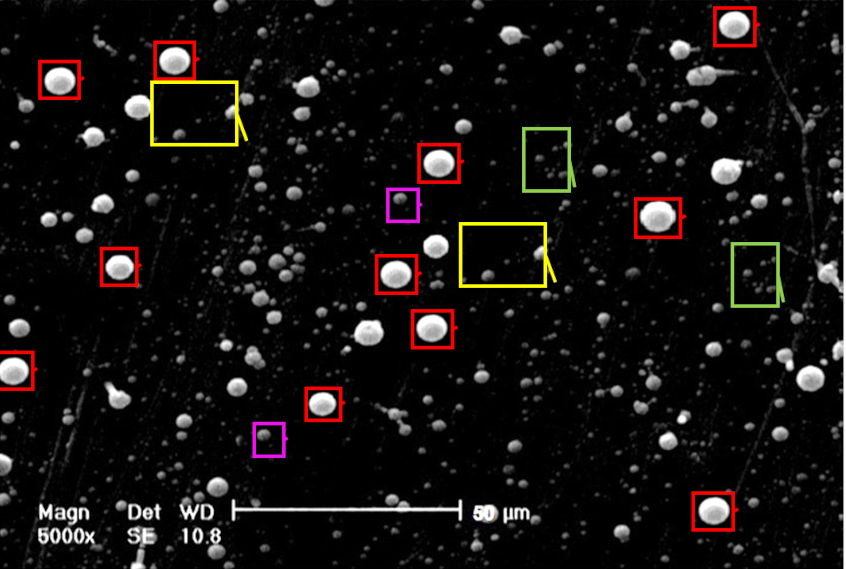
\includegraphics[width=0.8\textwidth]{img/pubpeer/pubpeer_dupes.png}
\end{figure}

\pagebreak
\begin{quote}
    \textit{Figure 6: Some of the images previously \href{https://pubpeer.com/publications/2E9CC5D00FDE41668A28B9622E64ED}{appeared elsewhere}. Identified by \href{https://imagetwin.ai}{Imagetwin.ai}.}
\end{quote}

\begin{figure}[h!tbp]
\centering
    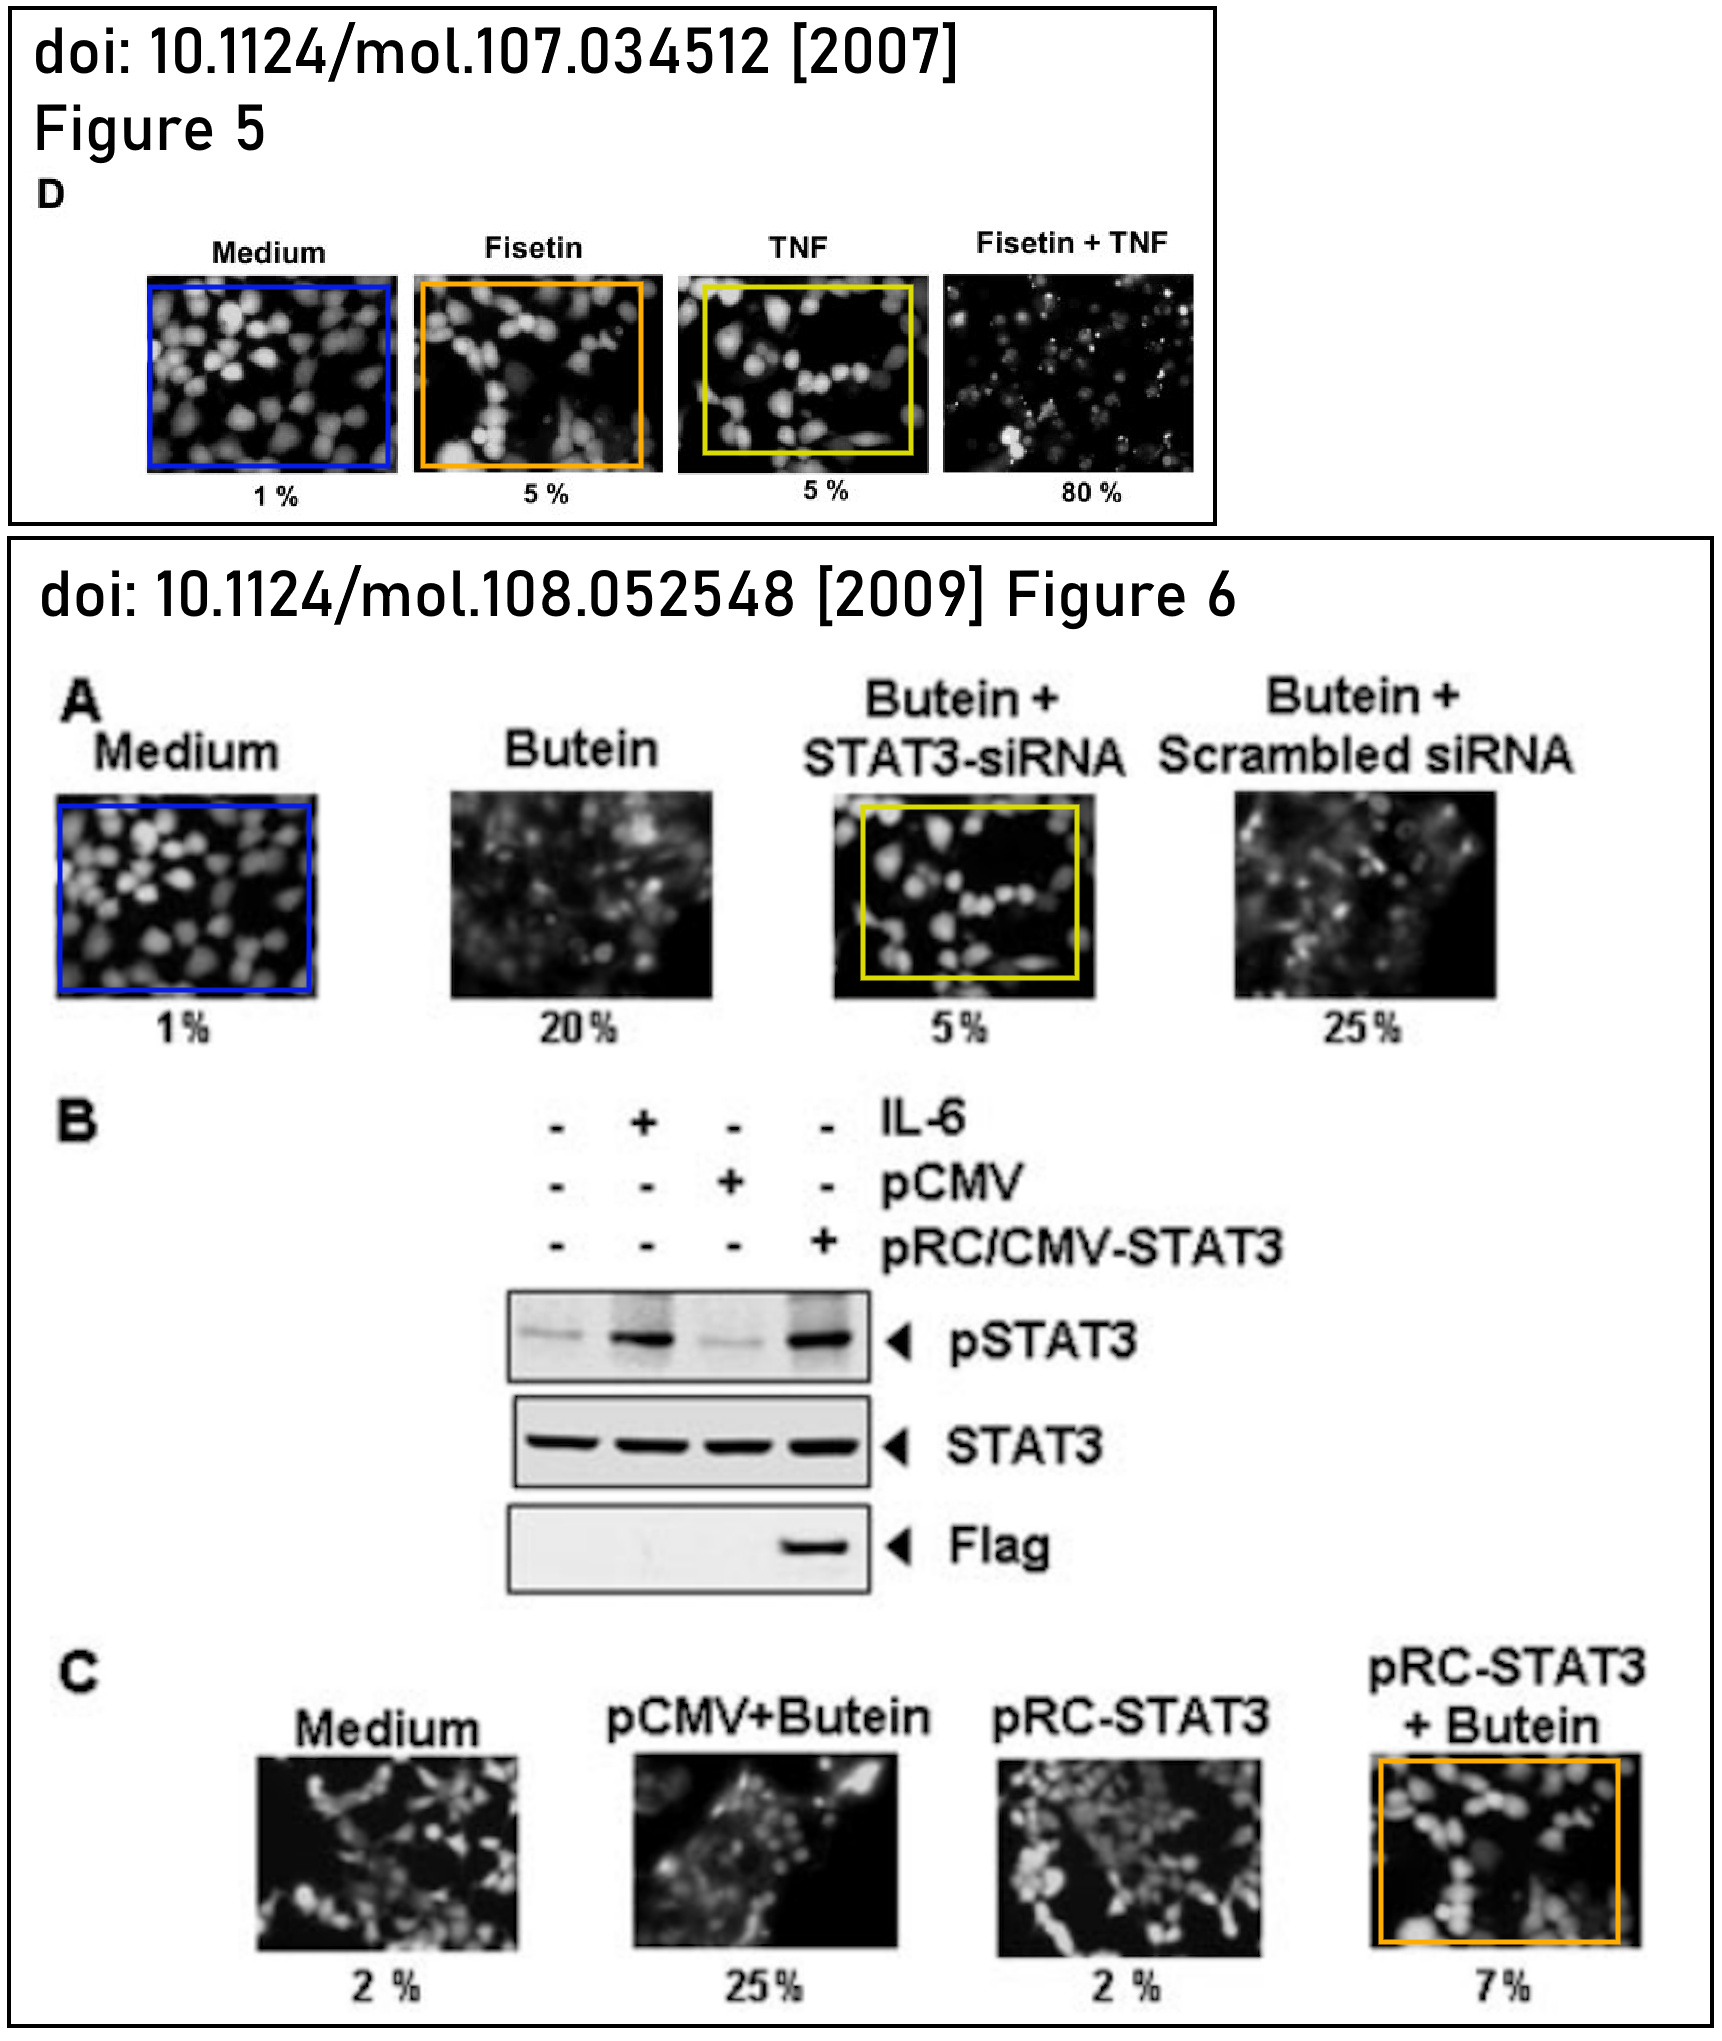
\includegraphics[width=0.5\textwidth]{img/pubpeer/image-1729709836291.png}
\end{figure}

\subsubsection*{Examples of unhelpful comments}

\begin{quote}
    \textit{The nanoparticles in Figure 8 look a bit wonky.}
\end{quote}

\begin{quote}
    \textit{Some of the lanes SDS-PAGE gel shown in Figure 4 look very similar to one another.}
\end{quote}

\subsection*{Do not speculate on researcher motivations}

Even when there is copious evidence that some fabrication, falsification or plagiarism occurred in a publication, it is not helpful to allege research misconduct. From the \href{https://pubpeer.com/static/faq#4}{PubPeer FAQ}:

\begin{quote}
    \textit{Allegations of misconduct are forbidden on PubPeer. They are anyway unnecessary. Your audience on the site is mostly composed of highly intelligent researchers and scientists. They are quite capable of drawing their own conclusions if the facts are clearly presented.}
\end{quote}

\begin{quote}
    \textit{You should also avoid personal comments about authors and speculation about researcher actions and motives. This is non-scientific, but also can pose legal problems.}
\end{quote}

Beyond this, it is often not possible to know exactly what took place in a publication's preparation and who was responsible for the improprieties observed in PubPeer comments.

\subsection*{Make specific, actionable requests from authors}

Authors are the best experts on their own publications and PubPeer has the option to provide author emails to loop them into a discussion. Questions about a publication can often be addressed directly by authors, so it is helpful to make clarifying requests where appropriate.

\begin{quote}
    \textit{Could the authors provide the original scanning electron microscope images shown in Figure 3?}
\end{quote}

\begin{quote}
    \textit{Could the authors provide the raw data for the EDX spectrum shown in Figure 4?}
\end{quote}

\begin{quote}
    \textit{Could the authors clarify how they estimated crystallite size?}
\end{quote}

\begin{quote}
    \textit{Could the authors clarify what ``enormous information'' means and why it was used instead of ``big data''?}
\end{quote}

\subsection*{Split multiple observations into multiple comments}

PubPeer comments can be referenced from other PubPeer comments on the same article by referring to the comment number preceded by ``\#''.

If you have many observations on different aspects of an article, consider splitting these observations into multiple comments so that other commenters can reference your specific observations one at a time.

\begin{figure}[h!tbp]
    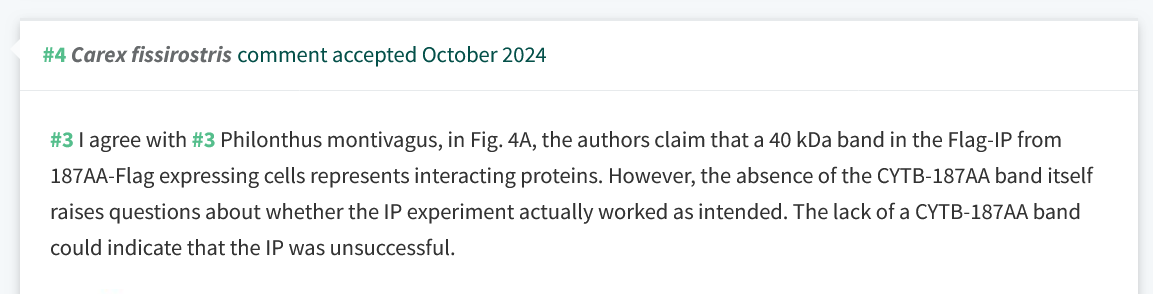
\includegraphics[width=\textwidth]{img/pubpeer/Screenshot 2024-10-23 at 16-36-04 PubPeer - A novel protein CYTB-187AA encoded by the mitochondrial gene.png}
    \caption*{This PubPeer comment refers back to a previous PubPeer comment using \#. The comment number for this comment can be found in the upper left corner of the comment box, to the left of the commenter's alias.}
\end{figure}
\end{document}
